%% Fall 2013 MDM Homework Template
\documentclass[12pt,letterpaper]{article}

\usepackage[utf8]{inputenc}
\usepackage[T1]{fontenc}
\usepackage{amsmath}
\usepackage{amsfonts}
\usepackage{amssymb}
\usepackage[left=2cm,right=2cm,top=2cm,bottom=2cm,headheight=22pt]{geometry}
\usepackage{fancyhdr}
\usepackage{setspace}
\usepackage{lastpage}
\usepackage{graphicx}

\begin{document}

%other parameters
\setlength{\parskip}{1ex plus 0.5ex minus 0.2ex}
\setlength{\parindent}{0pt}

%header and footer parameters
\pagestyle{fancy}
\lhead{Math 1100 section 03}
\chead{Weekly Homework}
\rhead{Due: 13 September}
\lfoot{}
\cfoot{\emph{Prof. Hitchman}}
\rfoot{}

\begin{center}
{
\Large
\textbf{Written Assignment \#3}
}
\end{center}

We have seen the following knot before, and noted that it is a planar projection of an unknot.
Show that this knot is equivalent to the unknot be describing a sequence of Reidemeister moves which change this planar projection into an ordinary circle.
Draw pictures of the steps along the way, and clearly label each transition with the type of move made.

\vspace{1cm}



\begin{figure}[h]
    \centering
    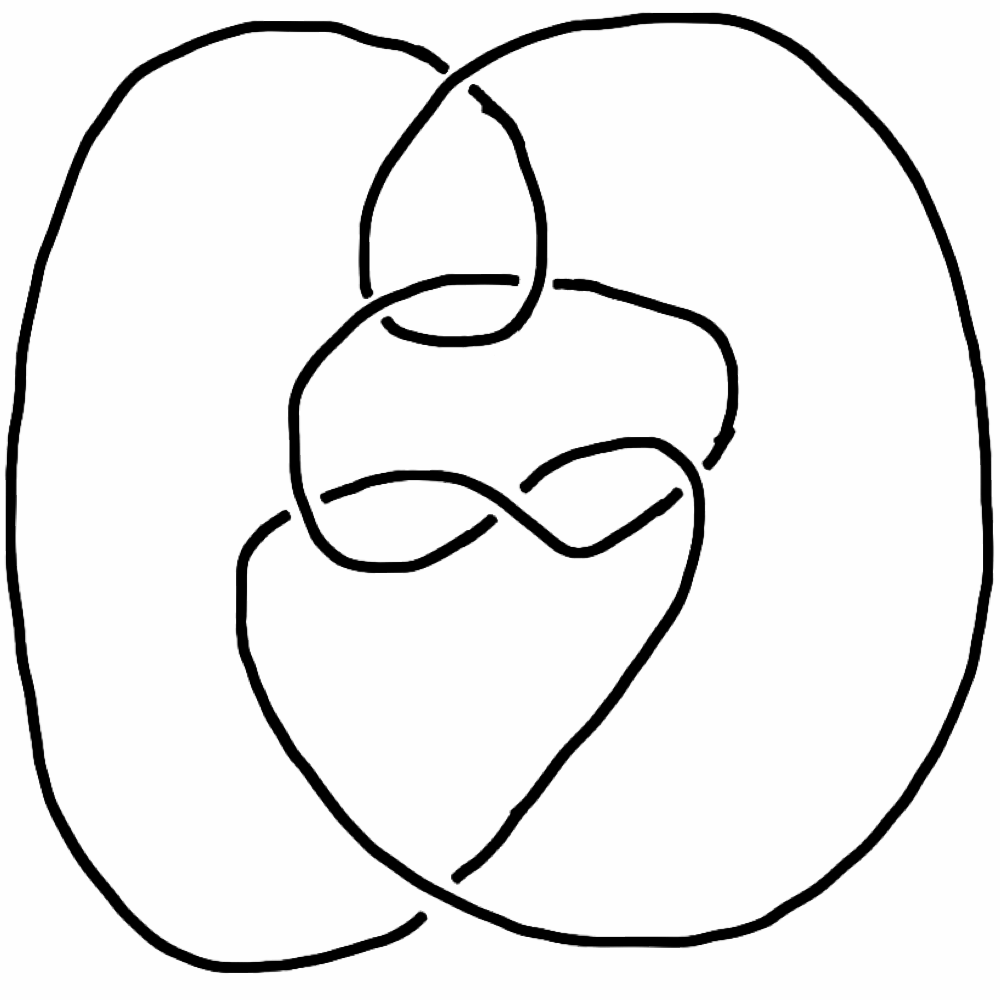
\includegraphics[width=.7\textwidth]{knotpics/9SeptQ5b.png}
    \caption{An Unknot}
\end{figure}




\end{document}
%sagemathcloud={"zoom_width":100}